\chapter{Discussion of Results} \label{chap:resul}

\section*{}

This chapter will discuss the results obtained in the first and second studies, proposed in the previous chapter.

\section{Study on Anomaly Detection Techniques}

\subsection{Performance}

Table~\ref{tab:best_algs} indicates the best techniques for each dataset according to the F1 metric, along with \textit{precision} and \textit{recall} metrics.
Different techniques (or the same technique with different parameter values) having the same F1 value for the same dataset are also listed.
On 11 (52\%) of the datasets the Random Forest technique was among the ones with higher F1, followed by the SVM (on 5 datasets).
However, in the case of the SVM, there was not a consensus on the best value for the \textit{kernel} parameter, which may become a disadvantage when using this technique for Anomaly Detection when compared to the Random Forest one.
It is also noticeable that all the techniques in Table~\ref{tab:best_algs} are supervised learning techniques, which supports the idea that this type of techniques have superior performance compared to the semi-supervised and unsupervised ones.

\begin{table}[!ht]
	\centering
	\caption{Measurements of the metrics F1, Precision and Recall for the algorithms with highest F1 in each dataset.}
	\label{tab:best_algs}
\begin{tabular}{@{}llllll@{}}
	\toprule
	\textbf{Dataset} & \textbf{Technique} & \textbf{Variant} & \textbf{F1} & \textbf{Precision} & \textbf{Recall} \\ \midrule
	ALOI & RF & - & 0.590 & 0.600 & 0.580 \\
	Ionosphere & SVM & kernel = radial & 0.933 & 0.929 & 0.937 \\
	KDDCup99 & RF & - & 0.852 & 0.854 & 0.850 \\
	PenDigits & MLP & - & 1.000 & 1.000 & 1.000 \\
	Shuttle & CART & - & 0.900 & 0.900 & 0.900 \\
	Waveform & SVM & kernel = radial & 0.600 & 0.600 & 0.600 \\
	WBC & RF & - & 0.900 & 0.900 & 0.900 \\
	WDBC & NB & - & 0.900 & 0.900 & 0.900 \\
	& MLP & - & 0.900 & 0.900 & 0.900 \\
	& SVM & kernel = linear & 0.900 & 0.900 & 0.900 \\
	& SVM & kernel = polynomial & 0.900 & 0.900 & 0.900 \\
	WPBC & SVM & kernel = linear & 0.536 & 0.520 & 0.555 \\
	Annthyroid & RF & - & 0.974 & 0.969 & 0.979 \\
	Arrhythmia & RF & - & 0.587 & 0.567 & 0.617 \\
	Cardiotocography & RF & - & 0.899 & 0.900 & 0.898 \\
	HeartDisease & NB & - & 0.650 & 0.625 & 0.683 \\
	Hepatitis & RF & - & 0.683 & 0.600 & 0.850 \\
	InternetAds & RF & - & 0.880 & 0.880 & 0.881 \\
	PageBlocks & RF & - & 0.885 & 0.886 & 0.884 \\
	Parkinson & SVM & kernel = linear & 0.917 & 0.950 & 0.900 \\
	& SVM & kernel = polynomial & 0.917 & 0.950 & 0.900 \\
	Pima & RF & - & 0.541 & 0.531 & 0.552 \\
	SpamBase & RF & - & 0.873 & 0.873 & 0.872 \\
	Stamps & MLP & - & 0.886 & 0.800 & 1.000 \\
	Wilt & MLP & - & 0.901 & 0.896 & 0.906 \\ \bottomrule
\end{tabular}
\end{table}

Table~\ref{tab:best_algs_semi} indicates the best semi-supervised techniques for each dataset.
The values of the F1 metric for this type of techniques are considerably lower, when compared to the ones on table~\ref{tab:best_algs}.
However, choosing of the value of the \textit{kernel} parameter for the One-class SVM technique appears to be easier than for the regular SVM, as on 86\% of the datasets the best value was \textit{radial}.

\begin{table}[!ht]
	\centering
	\caption{Measurements of the metrics F1, Precision and Recall for the semi-supervised algorithms with highest F1 in each dataset.}
	\label{tab:best_algs_semi}
\begin{tabular}{@{}llllll@{}}
	\toprule
	\textbf{Dataset} & \textbf{Technique} & \textbf{Variant} & \textbf{F1} & \textbf{Precision} & \textbf{Recall} \\ \midrule
	ALOI & One-class SVM & kernel = radial & 0.066 & 0.035 & 0.578 \\
	Ionosphere & One-class SVM & kernel = radial & 0.675 & 0.518 & 0.977 \\
	KDDCup99 & One-class SVM & kernel = radial & 0.016 & 0.008 & 1.000 \\
	PenDigits & One-class SVM & kernel = polynomial & 0.008 & 0.004 & 1.000 \\
	Shuttle & One-class SVM & kernel = radial & 0.049 & 0.025 & 1.000 \\
	Waveform & One-class SVM & kernel = radial & 0.087 & 0.046 & 0.810 \\
	WBC & One-class SVM & kernel = radial & 0.169 & 0.093 & 1.000 \\
	WDBC & One-class SVM & kernel = radial & 0.100 & 0.053 & 1.000 \\
	WPBC & One-class SVM & kernel = polynomial & 0.359 & 0.235 & 0.775 \\
	Annthyroid & One-class SVM & kernel = radial & 0.203 & 0.116 & 0.809 \\
	Arrhythmia & One-class SVM & kernel = radial & 0.273 & 0.163 & 0.883 \\
	Cardiotocography & One-class SVM & kernel = radial & 0.464 & 0.312 & 0.910 \\
	HeartDisease & One-class SVM & kernel = radial & 0.472 & 0.322 & 0.925 \\
	Hepatitis & One-class SVM & kernel = radial & 0.380 & 0.238 & 1.000 \\
	InternetAds & One-class SVM & kernel = radial & 0.398 & 0.261 & 0.843 \\
	PageBlocks & One-class SVM & kernel = radial & 0.294 & 0.172 & 0.996 \\
	Parkinson & One-class SVM & kernel = radial & 0.488 & 0.355 & 0.950 \\
	Pima & One-class SVM & kernel = radial & 0.397 & 0.270 & 0.753 \\
	SpamBase & One-class SVM & kernel = radial & 0.456 & 0.307 & 0.888 \\
	Stamps & One-class SVM & kernel = radial & 0.282 & 0.165 & 1.000 \\
	Wilt & One-class SVM & kernel = linear & 0.174 & 0.107 & 0.777 \\ \bottomrule
\end{tabular}
\end{table}

The results of the previous analysis for the unsupervised learning techniques are presented in table~\ref{tab:best_algs_un}.
The F1 values of this type of techniques are comparable to the ones from the semi-supervised techniques and therefore, lower that the ones on table~\ref{tab:best_algs}.
On 11 (52\%) of the datasets, the k-means technique had the best F1 value, followed by the LOF technique (7 datasets).

\begin{table}[!ht]
	\centering
	\caption{Measurements of the metrics F1, Precision and Recall for the unsupervised algorithms with highest F1 in each dataset.}
	\label{tab:best_algs_un}
	\begin{tabular}{@{}llllll@{}}
		\toprule
		\textbf{Dataset} & \textbf{Technique} & \textbf{Variant} & \textbf{F1} & \textbf{Precision} & \textbf{Recall} \\ \midrule
		ALOI & LOF & k = 3 & 0.207 & 0.207 & 0.207 \\
		Ionosphere & k-means & k = 25 & 0.849 & 0.849 & 0.849 \\
		KDDCup99 & k-means & k = 8 & 0.560 & 0.560 & 0.560 \\
		PenDigits & LOF & k = 3 & 0.050 & 0.050 & 0.050 \\
		& LOF & k = 5 & 0.050 & 0.050 & 0.050 \\
		& LOF & k = 8 & 0.050 & 0.050 & 0.050 \\
		& LOF & k = 14 & 0.050 & 0.050 & 0.050 \\
		& LOF & k = 19 & 0.050 & 0.050 & 0.050 \\
		Shuttle & DBSCAN & eps = 1.1 & 0.491 & 0.325 & 1.000 \\
		Waveform & k-means & k = 30 & 0.210 & 0.210 & 0.210 \\
		WBC & k-means & k = 19 & 0.600 & 0.600 & 0.600 \\
		WDBC & k-means & k = 30 & 0.700 & 0.700 & 0.700 \\
		& LOF & k = 19 & 0.700 & 0.700 & 0.700 \\
		WPBC & DBSCAN & eps = 0.3 & 0.384 & 0.237 & 1.000 \\
		& DBSCAN & eps = 0.5 & 0.384 & 0.237 & 1.000 \\
		& DBSCAN & eps = 0.7 & 0.384 & 0.237 & 1.000 \\
		& DBSCAN & eps = 0.9 & 0.384 & 0.237 & 1.000 \\
		& DBSCAN & eps = 1.1 & 0.384 & 0.237 & 1.000 \\
		Annthyroid & DBSCAN & eps = 1.1 & 0.190 & 0.122 & 0.438 \\
		Arrhythmia & k-means & k = 3 & 0.333 & 0.333 & 0.333 \\
		& LOF & k = 19 & 0.333 & 0.333 & 0.333 \\
		& LOF & k = 25 & 0.333 & 0.333 & 0.333 \\
		& LOF & k = 30 & 0.333 & 0.333 & 0.333 \\
		Cardiotocography & k-means & k = 3 & 0.364 & 0.364 & 0.364 \\
		HeartDisease & k-means & k = 14 & 0.351 & 0.351 & 0.351 \\
		& k-means & k = 30 & 0.351 & 0.351 & 0.351 \\
		Hepatitis & k-means & k = 25 & 0.308 & 0.308 & 0.308 \\
		& LOF & k = 25 & 0.308 & 0.308 & 0.308 \\
		& LOF & k = 30 & 0.308 & 0.308 & 0.308 \\
		InternetAds & LOF & k = 30 & 0.364 & 0.364 & 0.364 \\
		PageBlocks & k-means & k = 3 & 0.643 & 0.643 & 0.643 \\
		Parkinson & k-means & k = 8 & 0.667 & 0.667 & 0.667 \\
		& k-means & k = 14 & 0.667 & 0.667 & 0.667 \\
		Pima & DBSCAN & eps = 1.1 & 0.408 & 0.263 & 0.904 \\
		SpamBase & DBSCAN & eps = 1.1 & 0.339 & 0.204 & 0.991 \\
		Stamps & DBSCAN & eps = 1.1 & 0.310 & 0.183 & 1.000 \\
		Wilt & LOF & k = 5 & 0.152 & 0.152 & 0.152 \\ \bottomrule
	\end{tabular}
\end{table}

In some Anomaly Detection contexts, the \textit{precision} might be more important than \textit{recall} and vice-versa.
Therefore, an analysis on the best techniques according to the F0.5 and F2 metrics was also conducted.
Table~\ref{tab:best_algs_f05} lists the best techniques according to the F0.5 metric, in which \textit{precision} is favored.
In this case, the Random Forest technique is still considered the best one on most of the datasets (11).
Table~\ref{tab:best_algs_f20} lists the best techniques according to the F2.0 metric, in which \textit{recall} is favored.
Once again, the Random Forest technique is still considered the best one on most of the datasets (11). However, in this situation na unsupervised technique (DBSCAN) is the one with better performance on two datasets (WPBC and Pima).

\begin{table}[!ht]
	\centering
	\caption{Measurements of the metrics F0.5, Precision and Recall for the semi-supervised algorithms with highest F1 in each dataset.}
	\label{tab:best_algs_f05}
	\begin{tabular}{@{}llll@{}}
		\toprule
		\textbf{Dataset} & \textbf{Technique} & \textbf{Variant} & \textbf{F0.5} \\ \midrule
		ALOI & RF & - & 0.596 \\
		Ionosphere & SVM & kernel = radial & 0.931 \\
		KDDCup99 & RF & - & 0.854 \\
		PenDigits & MLP & - & 1.000 \\
		Shuttle & CART & - & 0.900 \\
		Waveform & SVM & kernel = radial & 0.600 \\
		WBC & RF & - & 0.900 \\
		WDBC & NB & - & 0.900 \\
		& MLP & - & 0.900 \\
		& SVM & kernel = linear & 0.900 \\
		& SVM & kernel = polynomial & 0.900 \\
		WPBC & SVM & kernel = linear & 0.526 \\
		Annthyroid & RF & - & 0.971 \\
		Arrhythmia & RF & - & 0.574 \\
		Cardiotocography & RF & - & 0.900 \\
		HeartDisease & NB & - & 0.634 \\
		Hepatitis & RF & - & 0.628 \\
		InternetAds & RF & - & 0.880 \\
		PageBlocks & RF & - & 0.886 \\
		Parkinson & SVM & kernel = linear & 0.933 \\
		& SVM & kernel = polynomial & 0.933 \\
		Pima & RF & - & 0.535 \\
		SpamBase & RF & - & 0.873 \\
		Stamps & MLP & - & 0.832 \\
		Wilt & MLP & - & 0.898 \\ \bottomrule
	\end{tabular}
\end{table}

\begin{table}[!ht]
	\centering
	\caption{Measurements of the metrics F2, Precision and Recall for the semi-supervised algorithms with highest F1 in each dataset.}
	\label{tab:best_algs_f20}
	\begin{tabular}{@{}llll@{}}
		\toprule
		\textbf{Dataset} & \textbf{Technique} & \textbf{Variant} & \textbf{F2} \\ \midrule
		ALOI & RF & - & 0.584 \\
		Ionosphere & SVM & kernel = radial & 0.936 \\
		KDDCup99 & RF & - & 0.851 \\
		PenDigits & MLP & - & 1.000 \\
		Shuttle & CART & - & 0.900 \\
		& RF & - & 0.900 \\
		& SVM & kernel = radial & 0.900 \\
		Waveform & SVM & kernel = radial & 0.600 \\
		WBC & RF & - & 0.900 \\
		WDBC & NB & - & 0.900 \\
		& MLP & - & 0.900 \\
		& SVM & kernel = linear & 0.900 \\
		& SVM & kernel = polynomial & 0.900 \\
		WPBC & DBSCAN & eps = 0.3 & 0.609 \\
		& DBSCAN & eps = 0.5 & 0.609 \\
		& DBSCAN & eps = 0.7 & 0.609 \\
		& DBSCAN & eps = 0.9 & 0.609 \\
		& DBSCAN & eps = 1.1 & 0.609 \\
		Annthyroid & RF & - & 0.977 \\
		Arrhythmia & RF & - & 0.603 \\
		Cardiotocography & RF & - & 0.898 \\
		HeartDisease & NB & - & 0.669 \\
		Hepatitis & RF & - & 0.767 \\
		InternetAds & RF & - & 0.880 \\
		PageBlocks & RF & - & 0.885 \\
		Parkinson & SVM & SVM\_linear & 0.906 \\
		& SVM & SVM\_polynomial & 0.906 \\
		Pima & DBSCAN & eps = 1.1 & 0.608 \\
		SpamBase & RF & - & 0.872 \\
		Stamps & MLP & - & 0.950 \\
		Wilt & MLP & - & 0.904 \\ \bottomrule
	\end{tabular}
\end{table}

Regarding the comparison between the Anomaly Detection techniques and the \textit{random} technique (that predicted every data instance randomly as \textit{anomalous} or not, taking into account class distribution), table~\ref{tab:better_than_random_datasets} lists the number of techniques (and its variants, considering the possible parameter values tested) that had a better F1 value than the \textit{random} technique.
The mean ratio of techniques with superior performance to the \textit{random} technique among the datasets is 0.83, while the minimum is 0.53.
In our experimental setup this indicates that in the worst case, only 53\% of the techniques were \textit{accurate}. However, given the fact that the mean among the datasets is considerably higher (83\%), we can conclude that we have a set of techniques in which the vast majority perform better than a random guess on most of the cases.
Table~\ref{tab:better_than_random_algorithms} reinforces this conclusion, by listing the number of datasets for each technique in which the technique (or one of its variants) outperformed the \textit{random} one.
Both the Random Forest and Multilayer Perceptron techniques outperformed the \textit{random} technique in every dataset, while the One-class SVM only did so in 71\% of the datasets.

\begin{table}[!ht]
	\centering
	\caption{Number of techniques (and each of its variants) that had a superior value on F1 metric to the \textit{random} technique in each dataset. The total number of techniques/variants tested was 31.}
	\label{tab:better_than_random_datasets}
	\begin{tabular}{@{}lll@{}}
		\toprule
		\textbf{Dataset} & \textbf{Variants better than random} & \textbf{Ratio} \\ \midrule
		ALOI & 30 & 0.94 \\
		Ionosphere & 29 & 0.91 \\
		KDDCup99 & 30 & 0.94 \\
		PenDigits & 20 & 0.63 \\
		Shuttle & 31 & 0.97 \\
		Waveform & 31 & 0.97 \\
		WBC & 18 & 0.56 \\
		WDBC & 21 & 0.66 \\
		WPBC & 17 & 0.53 \\
		Annthyroid & 31 & 0.97 \\
		Arrhythmia & 30 & 0.94 \\
		Cardiotocography & 29 & 0.91 \\
		HeartDisease & 27 & 0.84 \\
		Hepatitis & 24 & 0.75 \\
		InternetAds & 24 & 0.75 \\
		PageBlocks & 30 & 0.94 \\
		Parkinson & 29 & 0.91 \\
		Pima & 31 & 0.97 \\
		SpamBase & 29 & 0.91 \\
		Stamps & 31 & 0.97 \\
		Wilt & 18 & 0.56 \\ \bottomrule
	\end{tabular}
\end{table}

\begin{table}[!ht]
	\centering
	\caption{Number of datasets for which each technique had at least one variant with a better F1 value than the one from the \textit{random} technique.}
	\label{tab:better_than_random_algorithms}
	\begin{tabular}{@{}lll@{}}
		\toprule
		\textbf{Technique} & \textbf{Number of datasets} & \textbf{Ratio} \\ \midrule
		CART & 19 & 0.90 \\
		SVM & 18 & 0.86 \\
		NB & 17 & 0.81 \\
		RF & 21 & 1.00 \\
		MLP & 21 & 1.00 \\
		One-class SVM & 15 & 0.71 \\
		k-means & 19 & 0.90 \\
		DBSCAN & 20 & 0.95 \\
		LOF & 20 & 0.95 \\ \bottomrule
	\end{tabular}\
\end{table}

\subsection{Diversity}

Regarding the diversity of the techniques studied, figure~\ref{fig:mean} displays visually the mean value of the Jaccard metric, across all the 21 datasets tested and figure~\ref{fig:sd} the standard deviation value.
Figure~\ref{fig:mean} reveals visual \textit{clusters} of similarity between several techniques:

\begin{itemize}
	\item Supervised techniques are somewhat similar to each other but not similar to the semi-supervised and unsupervised ones;
	\item Semi-supervised techniques (One-class SVM) are more similar to each other and the DBSCAN technique, but display a very low degree of similarity to other techniques;
	\item The LOF technique's variants are very similar to each other (this similarity is higher if the variation of the parameter $k$ is lower) and somewhat similar to the k-means technique, but have a very low degree of similarity to other techniques;
	\item The DBSCAN technique's variants are very similar to each other (this similarity is higher if the variation of the parameter $eps$ is lower) and somewhat similar to the One-class SVM variants;
	\item The k-means technique's variants show a medium similarity to each other and to some variants of the LOF technique.
\end{itemize}

\begin{figure}[ht!]
	\centering
	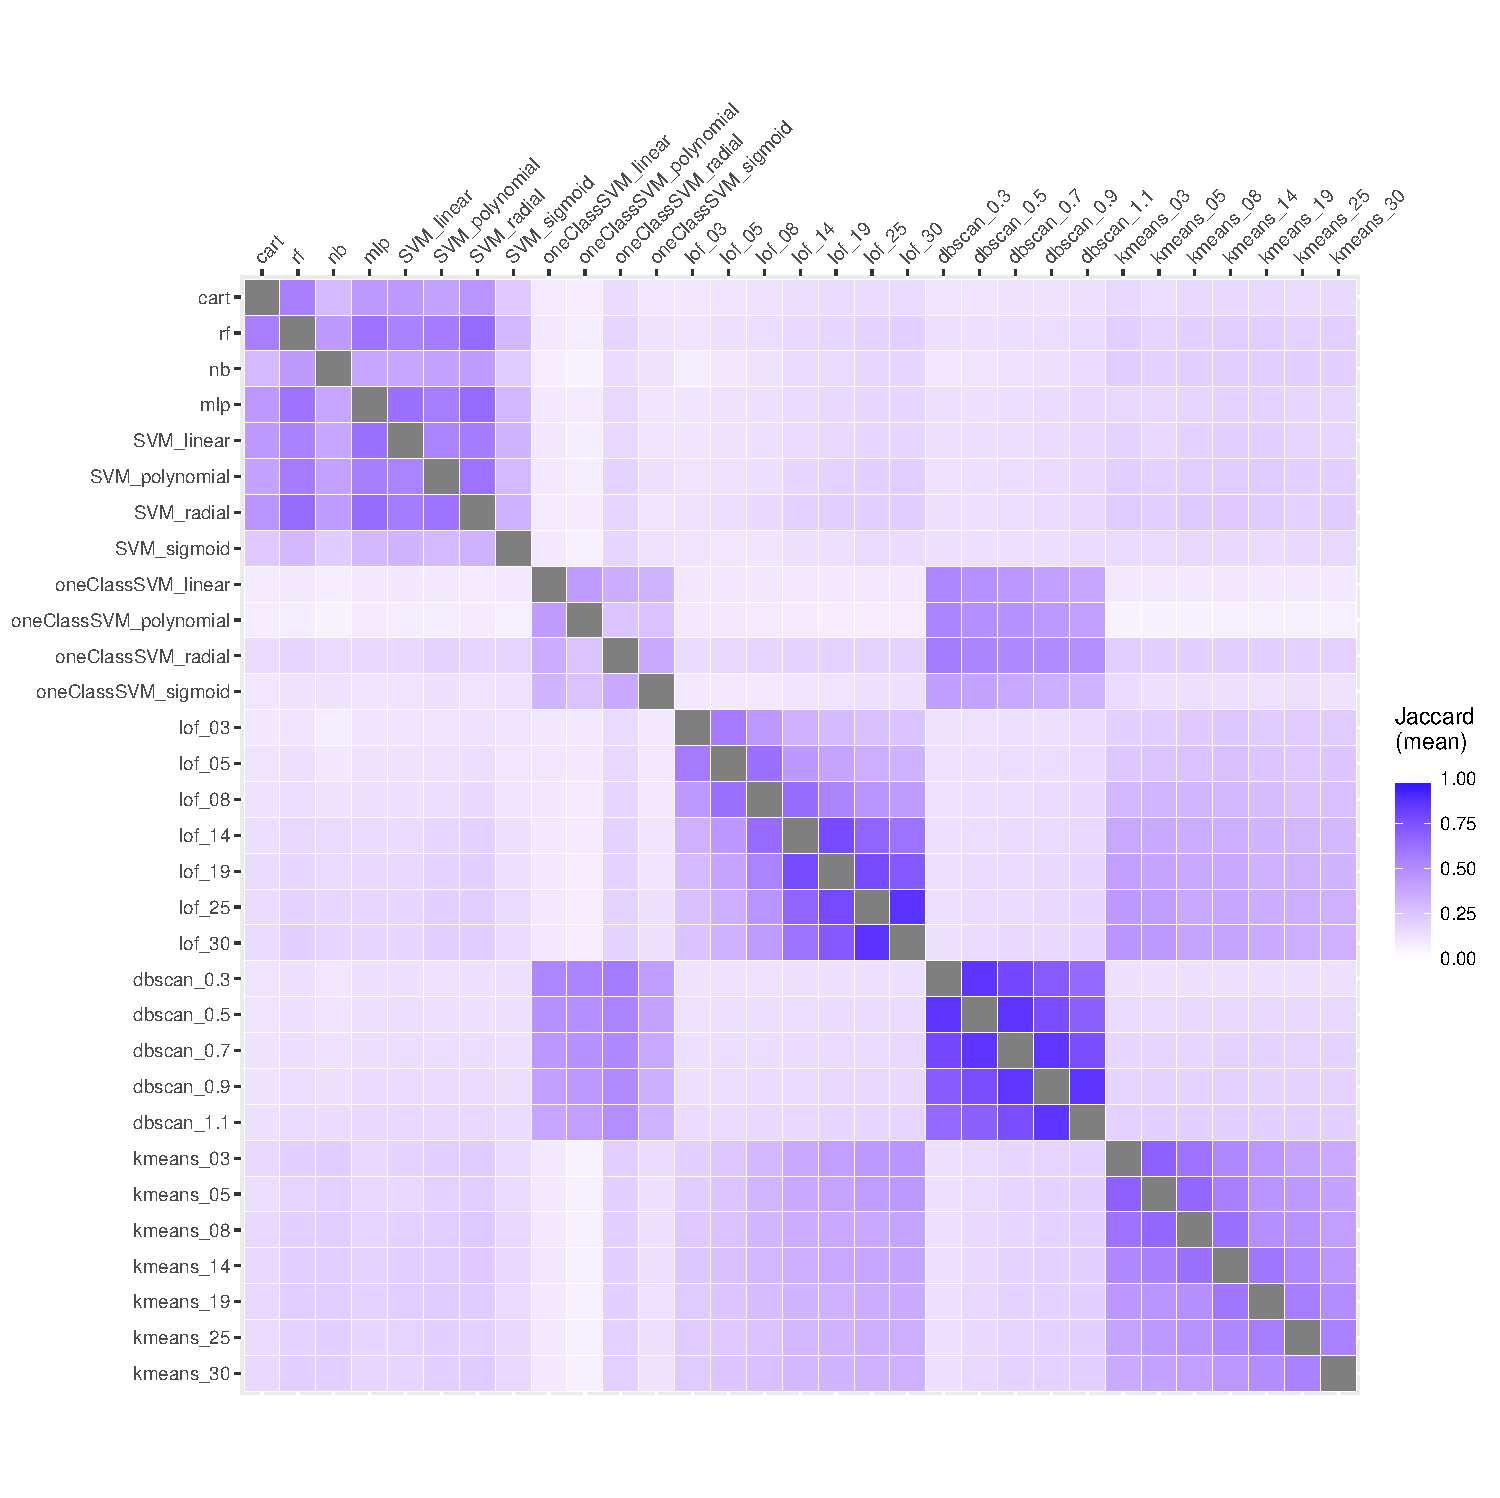
\includegraphics[width=\textwidth]{figures/plot_mean.pdf}
	\caption{Mean value across all datasets of the Jaccard metric between each par of techniques.}
	\label{fig:mean}
\end{figure}

Figure~\ref{fig:sd} show a more distinct variation on the similarity between the supervised learning techniques, between the DBSCAN technique's variations and between the DBSCAN's variations and one of the variations of the One-class SVM technique.

\begin{figure}[ht!]
	\centering
	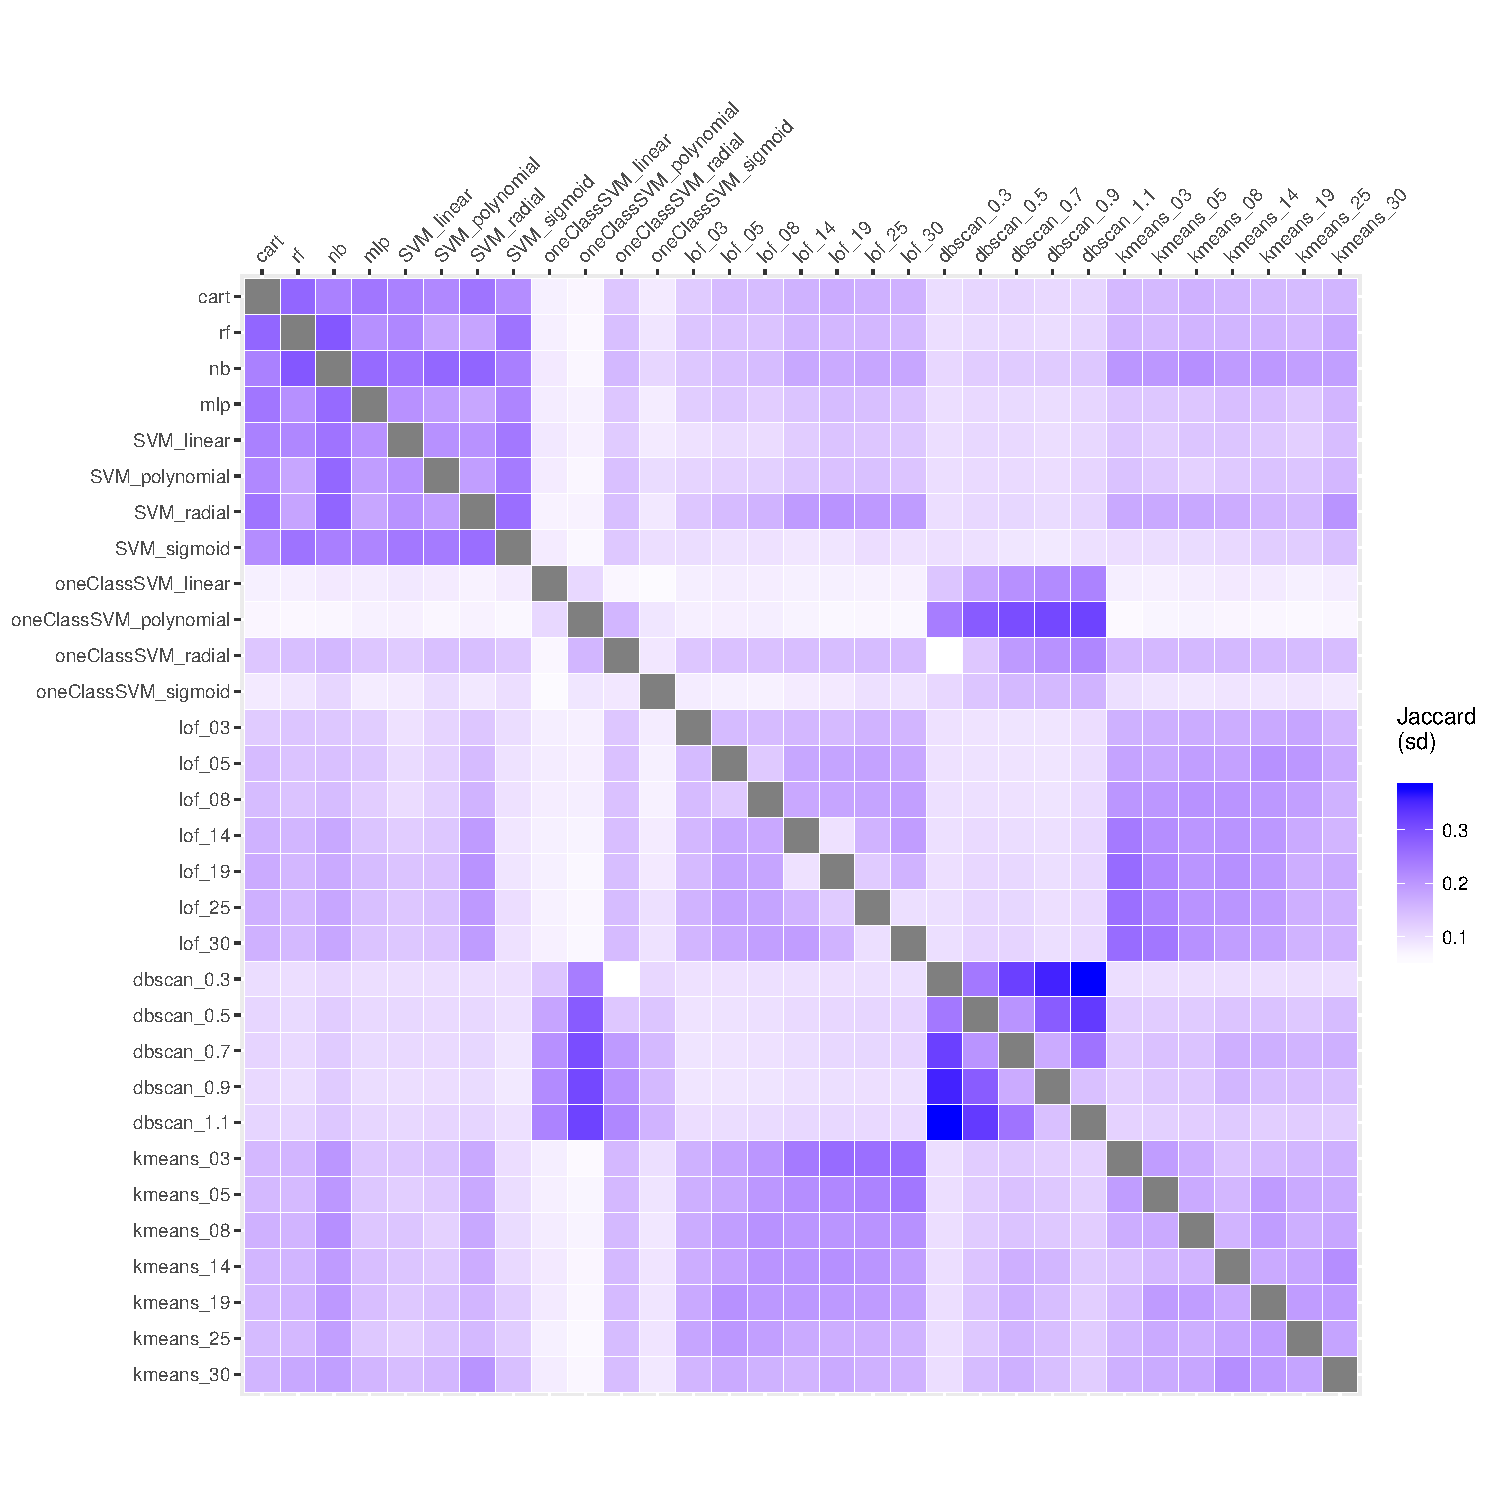
\includegraphics[width=\textwidth]{figures/plot_sd.pdf}
	\caption{Standard deviation value across all datasets of the Jaccard metric between each par of techniques.}
	\label{fig:sd}
\end{figure}

\section{Study on Stacking Approaches}

Table~\ref{tab:stacking_better_no_maj} lists the best Stacking approaches that outperformed the best single technique for each dataset.
In 12 of the 21 datasets there was an improvement in the F1's value over the best technique. The mean improvement in these 12 datasets was 0.025.

Regarding the techniques used in the ensemble, the best ensemble in 6 of the 12 datasets contained techniques from several learning modes: this is the case of the datasets ALOI, KDDCup99, WPBC, InternetAds, PageBlocks and Stamps.
In 5 of these 6 datasets, the best ensemble was the one that included all the techniques.
Given these results, there is not a clear conclusion on whether including techniques from different learning modes results in an ensemble with higher accuracy.

Regarding the best meta-classifier, there was not one that outperformed consistently all the others on the datasets used.

\begin{table}[!ht]
	\centering
	\caption{Measurements of the metric F1 for the Stacking approaches that outperform the best algorithm for each dataset.}
	\label{tab:stacking_better_no_maj}
	\resizebox{\textwidth}{!}{%
		\begin{tabular}{@{}llllll@{}}
			\toprule
			\textbf{Dataset} & \textbf{Ensemble Techniques} & \textbf{Meta-classifier} & \textbf{Best Technique F1} & \textbf{Best Ensemble F1} & \textbf{Improvement} \\ \midrule
			ALOI & All & RF & 0.933 & 0.947 & +0.014 \\
			KDDCup99 & All & RF & 0.852 & 0.879 & +0.027 \\
			Shuttle & One-class SVM + SVM & LR & 0.900 & 1.000 & +0.100 \\
			& One-class SVM + SVM & MLP & 0.900 & 1.000 & +0.100 \\
			& SVM & LR & 0.900 & 1.000 & +0.100 \\
			& SVM & MLP & 0.900 & 1.000 & +0.100 \\
			Waveform & SVM & CART & 0.600 & 0.640 & +0.040 \\
			WPBC & One-class SVM + SVM & MLP & 0.536 & 0.569 & +0.033 \\
			Annthyroid & All Supervised & CART & 0.974 & 0.976 & +0.002 \\
			Cardiotocography & All Supervised & CART & 0.899 & 0.905 & +0.006 \\
			HeartDisease & CART + RF & MLP & 0.650 & 0.672 & +0.022 \\
			InternetAds & All & LR & 0.880 & 0.898 & +0.018 \\
			PageBlocks & All & RF & 0.885 & 0.890 & +0.005 \\
			SpamBase & All Supervised & RF & 0.873 & 0.882 & +0.009 \\
			Stamps & All & CART & 0.886 & 0.906 & +0.020 \\ \bottomrule
	\end{tabular}}
\end{table}

Table~\ref{tab:stacking_better} lists the best Stacking approaches that outperformed the best single technique for each dataset, but this time considering additionally Majority Voting as an alternative to a meta-classifier.
Majority Voting is not a meta-classifier, so therefore a solution with it cannot be considered an application of the Stacking method.
However, the inclusion of Majority Voting can provide insight on whether how well the meta-classifiers are performing, by serving as a baseline.

In this case, in 15 of the 21 datasets there was an improvement of the F1's value over the best technique: more 3 datasets than without considering Majority Voting.
The mean value of this improvement was 0.056, also higher than the one from the previous experiment. The techniques included in most of the successful ensembles are the RF and CART algorithms, with Majority Voting being a better alternative to a meta-classifier in all datasets except Waveform and Stamps.

%Table~\ref{tab:stacking_better} lists the best Stacking approaches that outperformed the best single technique for each dataset. 
%The stacking approach outperformed the best individual technique in 15 of the 21 datasets, with the combination of the CART and Random Forest techniques as an ensemble and Majority Voting as a meta-classifier the most frequent combination (in 10 of the datasets).
%In most of the datasets, an ensemble of supervised learning techniques always outperformed an ensemble with techniques from several learning modes.
%Regarding the improvement observed, Stacking had a mean improvement of 0.0671 in the F1 metric's value

\begin{table}[!ht]
	\centering
	\caption{Measurements of the metric F1 for the Stacking approaches that outperform the best algorithm for each dataset, when considering Majority Voting as an alternative to a meta-classifier.}
	\label{tab:stacking_better}
	\resizebox{\textwidth}{!}{%
\begin{tabular}{@{}llllll@{}}
	\toprule
	\textbf{Dataset} & \textbf{Ensemble Techniques} & \textbf{Meta-classifier} & \textbf{Best Technique F1} & \textbf{Best Ensemble F1} & \textbf{Improvement} \\ \midrule
	ALOI & CART + RF & Majority Voting & 0.590 & 0.742 & +0.152 \\
	Ionosphere & DBSCAN & Majority Voting & 0.933 & 1.000 & +0.067 \\
	KDDCup99 & CART + RF & Majority Voting & 0.852 & 0.892 & +0.040 \\
	Shuttle & All Supervised & Majority Voting & 0.900 & 1.000 & +0.100 \\
	 & One-class SVM + SVM & LR & 0.900 & 1.000 & +0.100 \\
	 & One-class SVM + SVM & MLP & 0.900 & 1.000 & +0.100 \\
	 & SVM & Majority Voting & 0.900 & 1.000 & +0.100 \\
	 & SVM & LR & 0.900 & 1.000 & +0.100 \\
	 & SVM & MLP & 0.900 & 1.000 & +0.100 \\
	Waveform & SVM & CART & 0.600 & 0.640 & +0.040 \\
	WPBC & CART + RF & Majority Voting & 0.536 & 0.625 & +0.089 \\
	Annthyroid & CART + RF & Majority Voting & 0.974 & 0.979 & +0.005 \\
	Arrhythmia & CART + RF & Majority Voting & 0.587 & 0.653 & +0.066 \\
	Cardiotocography & CART + RF & Majority Voting & 0.899 & 0.928 & +0.029 \\
	HeartDisease & CART + RF & Majority Voting & 0.650 & 0.676 & +0.026 \\
	InternetAds & All Supervised & Majority Voting & 0.880 & 0.913 & +0.032 \\
	PageBlocks & CART + RF & Majority Voting & 0.885 & 0.919 & +0.034 \\
	Pima & CART + RF & Majority Voting & 0.541 & 0.647 & +0.106 \\
	SpamBase & CART + RF & Majority Voting & 0.873 & 0.908 & +0.036 \\
	Stamps & All & CART & 0.886 & 0.906 & +0.020 \\ \bottomrule
\end{tabular}}
\end{table}

%It might be somewhat debatable if the Majority Voting can be considered a simpler Stacking approach. Therefore, the results of this study without the Majority Voting algorithm being considered as a meta-classifier are displayed in table~\ref{tab:stacking_better_no_maj}
%In this case, in 12 of the 21 datasets there was an improvement in the F1's value over the best technique.
%Regarding the techniques used in the ensemble, once again there was no benefit in using \textit{hybrid} ensemble with techniques from several learning modes.

